%------------------------------------------------------------------------------
%
% Repository path   : $HeadURL: https://hbergauer@forge.hephy.oeaw.ac.at/scm/svn/project-cmstrigger/GlobalTriggerUpgrade/doc/latex/gt-mp7-firmware-specification/content/com-hardware.tex $
% Last committed    : $Revision: 2885 $
% Last changed by   : $Author: rahbaran $
% Last changed date : $Date: 2014-04-23 13:41:33 +0200 (Wed, 23 Apr 2014) $
% Description       : common Hardware Components
% ------------------------------------------------------------------------------


\clearpage



\subsubsection{Optical "splitting" of \ugt input data}\label{sec:gtl:optical_spliting_input_data}
The "splitting" of the \ugt input data (from \ugmt, Calo L2 and the external conditions) could be done in certain MP7 modules of \ugt. If there are more than 6 used \ugt modules,
Calo L2 and \ugmt are not able to provide the "splitted" data to \ugt. Therefore a set of used \ugt modules receives a certain number of fibers and split it over the TX.1 and TX.2 connections
via an optical patch-panel to the RX.1 connections of all used \ugt modules. Therefore we need an additional optical patch-panel to that, which is described in chapter \ref{sec:com-hard:fiber_optic_patch_gt_crate},
the design of the connections is not done yet.\\
For example: at the moment we have 8 fibers from Calo L2, 4 fibers from \ugmt and 2 fibers for external conditions (all with 10 Gb/s data rate), so in total 14 fibers.
Let's imagine, that we use 36 \ugt modules (!), we need 7 of the 36 modules to split the \ugt input data, every of the 7 modules can split 2 fibers (with input data) 36 times (!),
because of 72 transmitters (on TX.1 and TX.2). Therefore we need an additional optical patch-panel.

\subsection{Fiber Optic Patch Panels for \ugt-crate}\label{sec:com-hard:fiber_optic_patch_gt_crate}

\ugt patch panel is Rack mount 4U fiber optic patch panel, loaded with 36 MAC1410G (2x multimode (OM3, aqua color) duplex LC) panels.
It is loaded with (36) MAC1410G panels Total of 72 LC ports (144 fiber ports) 4U High (7").

The connector panel accepts modular adapter caps so the enclosure can be field configured with any
type standard fiber optic adapter. The connector panel is recessed 4.75” from front door to provide ample
room and bend radius management for patch cords and connectors. 


Figure \ref{fig:com-hard:mGT_mGMT_fiber_optical_patch} shows the overview of connection, which comes from Calo L2 (DeMux:mGT), Calo L2 (DeMux:mGMT) as well as from: barrel (TF), Overlap (TF) and Forward (TF). 
As output patch panel delivers objects for 6 \ugt cards, one \ugmt. 

\ugt patch panel is designed for getting the objects via fiber over LC connectors. 

This is the short overview the input/output of patch panel.

\begin{itemize}
\item Inputs: 144 LC connectors
\item Outputs: 8 * (MTP48 to LC 36 fiber OM3/4 Data Center Harness), which each LC on this cable can be configured. 
\item free LCs: it depends on which configuration, which we use. If we use 4 LC connectors for Legacy RPC, we have 16 LC free connectors as input. If we used
overlap TF instead of legacy RPCs, we have 8 LCs free as input. 
\end{itemize}


\begin{figure}[htb]
\centering
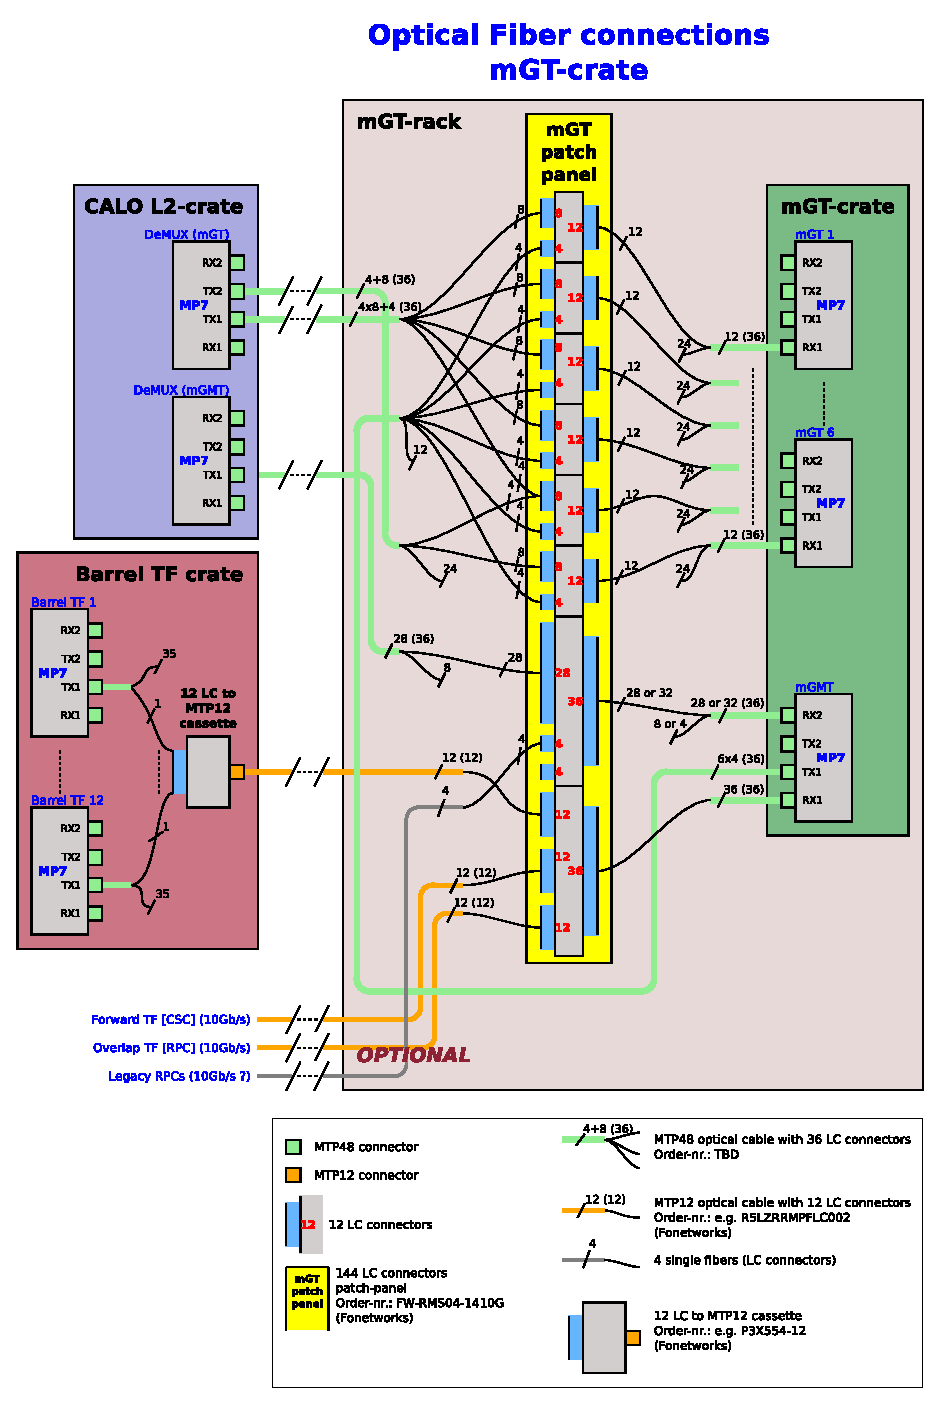
\includegraphics[width=14cm]{figures/mGT_mGMT_optical_connections}
\caption{Optical connections \ugt-crate} 
\label{fig:com-hard:mGT_mGMT_fiber_optical_patch}
\end{figure}

\clearpage

Figure \ref{fig:com-hard:mGT_mGMT_144_LC_patch_panel} shows the front panel of the patch panel - \textbf{first draft}.

\begin{figure}[htb]
\centering
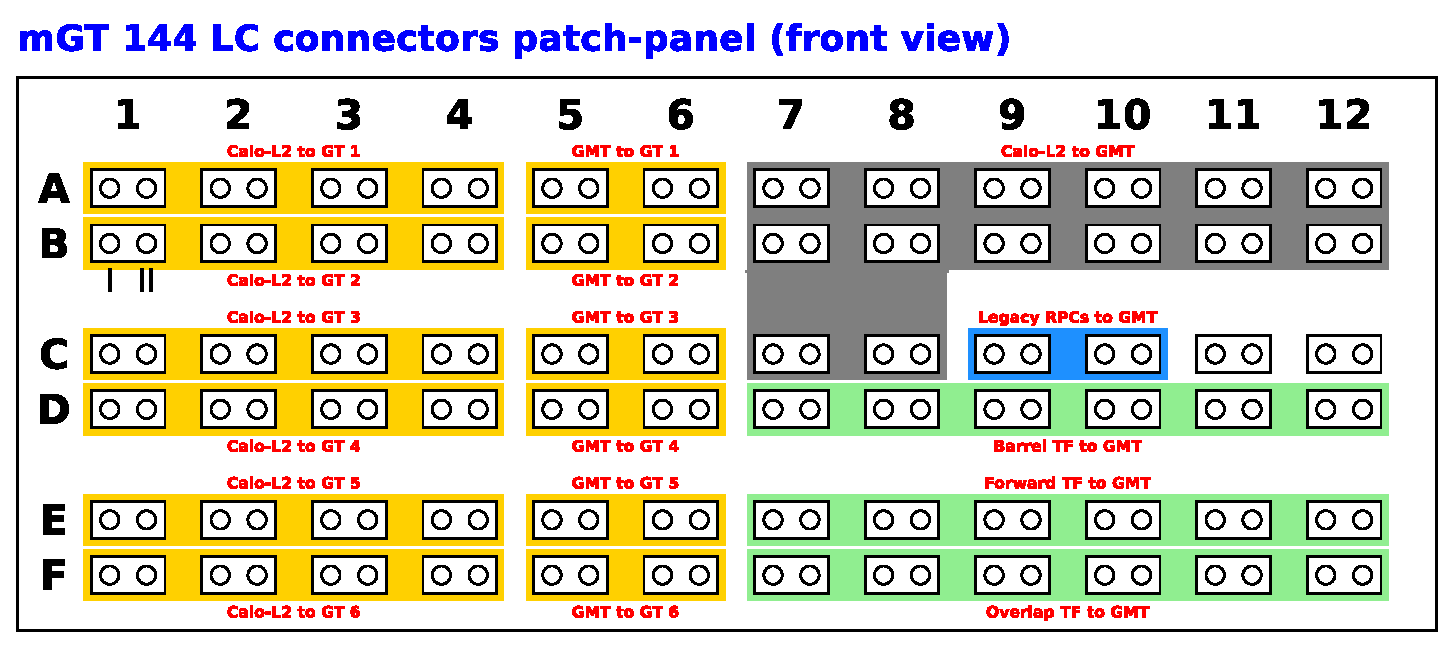
\includegraphics[width=14cm]{figures/mGT_mGMT_144_LC_patch_panel}
\caption{Optical patch-panel \ugt-crate (front view)} 
\label{fig:com-hard:mGT_mGMT_144_LC_patch_panel}
\end{figure}

\clearpage

Figures \ref{fig:com-hard:mGT_crate_optical_pp_connections} and \ref{fig:com-hard:mGT_crate_optical_pp_connections_2} 
show patching the LC connectors - \textbf{first draft}.

\begin{figure}[htb]
\centering
\includegraphics[width=14cm]{figures/mGT_crate_optical_pp_connections}
\caption{Optical connections on patch-panel \ugt-crate (part 1)} 
\label{fig:com-hard:mGT_crate_optical_pp_connections}
\end{figure}

\begin{figure}[htb]
\centering
\includegraphics[width=14cm]{figures/mGT_crate_optical_pp_connections_2}
\caption{Optical connections on patch-panel \ugt-crate (part 2)} 
\label{fig:com-hard:mGT_crate_optical_pp_connections_2}
\end{figure}

\clearpage

% Table \ref{tab:com-hard:mGT_mGMT_optical_connections_table} shows patching the LC connectors - \textbf{first draft}, has to be renewed because of Calo-L2 fiber connections.
% 
% \begin{longtable}{|p{.09\columnwidth}|p{.1\columnwidth}|p{.08\columnwidth}|p{.1\columnwidth}|p{.2\columnwidth}|p{.07\columnwidth}|p{.07\columnwidth}|p{.07\columnwidth}|}\hline 
% \textbf{Source mod. conn.} & \textbf{Source cable name} & \textbf{Source fiber} & \textbf{mGT patch-panel location} & \textbf{Data on fiber} & \textbf{Dest. fiber} & \textbf{Dest. cable name} & \textbf{Dest. mod. conn.}\\\hline\hline 
% \endhead
% \multirow{8}{16mm}{Calo-L2 DeMUX \ugt TX1} & \multirow{8}{15mm}{CALO 1} & 1  & A-1-I   & \egamma 0..5  & 1  & \multirow{12}{12mm}{GT 1} & \multirow{12}{12mm}{\ugt board 1 RX1}\\\cline{3-6}
%                                            &                            & 2  & A-1-II  & \egamma 6..11 & 2  &                           &                                      \\\cline{3-6}
%                                            &                            & 3  & A-2-I   & jet 0..5      & 3  &                           &                                      \\\cline{3-6}
%                                            &                            & 4  & A-2-II  & jet 6..11     & 4  &                           &                                      \\\cline{3-6}
%                                            &                            & 5  & A-3-I   & tau 0..5      & 5  &                           &                                      \\\cline{3-6}
%                                            &                            & 6  & A-3-II  & tau 6..11     & 6  &                           &                                      \\\cline{3-6}
%                                            &                            & 7  & A-4-I   & energy sums   & 7  &                           &                                      \\\cline{3-6}
%                                            &                            & 8  & A-4-II  & "not used"    & 8  &                           &                                      \\\cline{1-6}
% \multirow{4}{16mm}{\ugmt TX1}              & \multirow{4}{15mm}{GMT 3}  & 1  & A-5-I   & muon 0..1     & 9  &                           &                                      \\\cline{3-6}
%                                            &                            & 2  & A-5-II  & muon 2..3     & 10 &                           &                                      \\\cline{3-6}
%                                            &                            & 3  & A-6-I   & muon 4..5     & 11 &                           &                                      \\\cline{3-6}
%                                            &                            & 4  & A-6-II  & muon 6..7     & 12 &                           &                                      \\\hline
% \multirow{8}{16mm}{Calo-L2 DeMUX \ugt TX1} & \multirow{8}{15mm}{CALO 1} & 9  & B-1-I   & \egamma 0..5  & 1  & \multirow{12}{12mm}{GT 2} & \multirow{12}{12mm}{\ugt board 2 RX1}\\\cline{3-6}
%                                            &                            & 10 & B-1-II  & \egamma 6..11 & 2  &                           &                                      \\\cline{3-6}
%                                            &                            & 11 & B-2-I   & jet 0..5      & 3  &                           &                                      \\\cline{3-6}
%                                            &                            & 12 & B-2-II  & jet 6..11     & 4  &                           &                                      \\\cline{3-6}
%                                            &                            & 13 & B-3-I   & tau 0..5      & 5  &                           &                                      \\\cline{3-6}
%                                            &                            & 14 & B-3-II  & tau 6..11     & 6  &                           &                                      \\\cline{3-6}
%                                            &                            & 15 & B-4-I   & energy sums   & 7  &                           &                                      \\\cline{3-6}
%                                            &                            & 16 & B-4-II  & "not used"    & 8  &                           &                                      \\\cline{1-6}
% \multirow{4}{16mm}{\ugmt TX1}              & \multirow{4}{15mm}{GMT 3}  & 5  & B-5-I   & muon 0..1     & 9  &                           &                                      \\\cline{3-6}
%                                            &                            & 6  & B-5-II  & muon 2..3     & 10 &                           &                                      \\\cline{3-6}
%                                            &                            & 7  & B-6-I   & muon 4..5     & 11 &                           &                                      \\\cline{3-6}
%                                            &                            & 8  & B-6-II  & muon 6..7     & 12 &                           &                                      \\\hline
% \multirow{8}{16mm}{Calo-L2 DeMUX \ugt TX1} & \multirow{8}{15mm}{CALO 1} & 17 & C-1-I   & \egamma 0..5  & 1  & \multirow{12}{12mm}{GT 3} & \multirow{12}{12mm}{\ugt board 3 RX1}\\\cline{3-6}
%                                            &                            & 18 & C-1-II  & \egamma 6..11 & 2  &                           &                                      \\\cline{3-6}
%                                            &                            & 19 & C-2-I   & jet 0..5      & 3  &                           &                                      \\\cline{3-6}
%                                            &                            & 20 & C-2-II  & jet 6..11     & 4  &                           &                                      \\\cline{3-6}
%                                            &                            & 21 & C-3-I   & tau 0..5      & 5  &                           &                                      \\\cline{3-6}
%                                            &                            & 22 & C-3-II  & tau 6..11     & 6  &                           &                                      \\\cline{3-6}
%                                            &                            & 23 & C-4-I   & energy sums   & 7  &                           &                                      \\\cline{3-6}
%                                            &                            & 24 & C-4-II  & "not used"    & 8  &                           &                                      \\\cline{1-6}
% \multirow{4}{16mm}{\ugmt TX1}              & \multirow{4}{15mm}{GMT 3}  & 9  & C-5-I   & muon 0..1     & 9  &                           &                                      \\\cline{3-6}
%                                            &                            & 10 & C-5-II  & muon 2..3     & 10 &                           &                                      \\\cline{3-6}
%                                            &                            & 11 & C-6-I   & muon 4..5     & 11 &                           &                                      \\\cline{3-6}
%                                            &                            & 12 & C-6-II  & muon 6..7     & 12 &                           &                                      \\\hline
% \multirow{8}{16mm}{Calo-L2 DeMUX \ugt TX1} & \multirow{8}{15mm}{CALO 1} & 25 & D-1-I   & \egamma 0..5  & 1  & \multirow{12}{12mm}{GT 4} & \multirow{12}{12mm}{\ugt board 4 RX1}\\\cline{3-6}
%                                            &                            & 26 & D-1-II  & \egamma 6..11 & 2  &                           &                                      \\\cline{3-6}
%                                            &                            & 27 & D-2-I   & jet 0..5      & 3  &                           &                                      \\\cline{3-6}
%                                            &                            & 28 & D-2-II  & jet 6..11     & 4  &                           &                                      \\\cline{3-6}
%                                            &                            & 29 & D-3-I   & tau 0..5      & 5  &                           &                                      \\\cline{3-6}
%                                            &                            & 30 & D-3-II  & tau 6..11     & 6  &                           &                                      \\\cline{3-6}
%                                            &                            & 31 & D-4-I   & energy sums   & 7  &                           &                                      \\\cline{3-6}
%                                            &                            & 32 & D-4-II  & "not used"    & 8  &                           &                                      \\\cline{1-6}
% \multirow{4}{16mm}{\ugmt TX1}              & \multirow{4}{15mm}{GMT 3}  & 13 & D-5-I   & muon 0..1     & 9  &                           &                                      \\\cline{3-6}
%                                            &                            & 14 & D-5-II  & muon 2..3     & 10 &                           &                                      \\\cline{3-6}
%                                            &                            & 15 & D-6-I   & muon 4..5     & 11 &                           &                                      \\\cline{3-6}
%                                            &                            & 16 & D-6-II  & muon 6..7     & 12 &                           &                                      \\\hline
% \multirow{4}{16mm}{Calo-L2 DeMUX \ugt TX1} & \multirow{4}{15mm}{CALO 1} & 33 & E-1-I   & \egamma 0..5  & 1  & \multirow{12}{12mm}{GT 5} & \multirow{12}{12mm}{\ugt board 5 RX1}\\\cline{3-6}
%                                            &                            & 34 & E-1-II  & \egamma 6..11 & 2  &                           &                                      \\\cline{3-6}
%                                            &                            & 35 & E-2-I   & jet 0..5      & 3  &                           &                                      \\\cline{3-6}
%                                            &                            & 36 & E-2-II  & jet 6..11     & 4  &                           &                                      \\\cline{1-6}
% \multirow{4}{16mm}{Calo-L2 DeMUX \ugt TX2} & \multirow{4}{15mm}{CALO 2} & 1  & E-3-I   & tau 0..5      & 5  &                           &                                      \\\cline{3-6}
%                                            &                            & 2  & E-3-II  & tau 6..11     & 6  &                           &                                      \\\cline{3-6}
%                                            &                            & 3  & E-4-I   & energy sums   & 7  &                           &                                      \\\cline{3-6}
%                                            &                            & 4  & E-4-II  & "not used"    & 8  &                           &                                      \\\cline{1-6}
% \multirow{4}{16mm}{\ugmt TX1}              & \multirow{4}{15mm}{GMT 3}  & 17 & E-5-I   & muon 0..1     & 9  &                           &                                      \\\cline{3-6}
%                                            &                            & 18 & E-5-II  & muon 2..3     & 10 &                           &                                      \\\cline{3-6}
%                                            &                            & 19 & E-6-I   & muon 4..5     & 11 &                           &                                      \\\cline{3-6}
%                                            &                            & 20 & E-6-II  & muon 6..7     & 12 &                           &                                      \\\hline
% \multirow{8}{16mm}{Calo-L2 DeMUX \ugt TX2} & \multirow{8}{15mm}{CALO 2} & 5  & F-1-I   & \egamma 0..5  & 1  & \multirow{12}{12mm}{GT 6} & \multirow{12}{12mm}{\ugt board 6 RX1}\\\cline{3-6}
%                                            &                            & 6  & F-1-II  & \egamma 6..11 & 2  &                           &                                      \\\cline{3-6}
%                                            &                            & 7  & F-2-I   & jet 0..5      & 3  &                           &                                      \\\cline{3-6}
%                                            &                            & 8  & F-2-II  & jet 6..11     & 4  &                           &                                      \\\cline{3-6}
%                                            &                            & 9  & F-3-I   & tau 0..5      & 5  &                           &                                      \\\cline{3-6}
%                                            &                            & 10 & F-3-II  & tau 6..11     & 6  &                           &                                      \\\cline{3-6}
%                                            &                            & 11 & F-4-I   & energy sums   & 7  &                           &                                      \\\cline{3-6}
%                                            &                            & 12 & F-4-II  & "not used"    & 8  &                           &                                      \\\cline{1-6}
% \multirow{4}{16mm}{\ugmt TX1}              & \multirow{4}{15mm}{GMT 3}  & 21 & F-5-I   & muon 0..1     & 9  &                           &                                      \\\cline{3-6}
%                                            &                            & 22 & F-5-II  & muon 2..3     & 10 &                           &                                      \\\cline{3-6}
%                                            &                            & 23 & F-6-I   & muon 4..5     & 11 &                           &                                      \\\cline{3-6}
%                                            &                            & 24 & F-6-II  & muon 6..7     & 12 &                           &                                      \\\hline
% \multirow{28}{16mm}{Calo-L2 DeMUX \ugmt TX1} & \multirow{28}{15mm}{CALO 3} & 1  & A-7-I   & \multirow{28}{30mm}{???}       & 1  & \multirow{36}{15mm}{GMT 2} & \multirow{36}{12mm}{\ugmt RX2}     \\\cline{3-4}\cline{6-6}
%                                              &                             & 2  & A-7-II  &            & 2  &                           &                                    \\\cline{3-4}\cline{6-6}
%                                              &                             & 3  & A-8-I   &            & 3  &                           &                                    \\\cline{3-4}\cline{6-6}
%                                              &                             & 4  & A-8-II  &            & 4  &                           &                                    \\\cline{3-4}\cline{6-6}
%                                              &                             & 5  & A-9-I   &            & 5  &                           &                                    \\\cline{3-4}\cline{6-6}
%                                              &                             & 6  & A-9-II  &            & 6  &                           &                                    \\\cline{3-4}\cline{6-6}
%                                              &                             & 7  & A-10-I  &            & 7  &                           &                                    \\\cline{3-4}\cline{6-6}
%                                              &                             & 8  & A-10-II &            & 8  &                           &                                    \\\cline{3-4}\cline{6-6}
%                                              &                             & 9  & A-11-I  &            & 9  &                           &                                    \\\cline{3-4}\cline{6-6}
%                                              &                             & 10 & A-11-II &            & 10 &                           &                                    \\\cline{3-4}\cline{6-6}
%                                              &                             & 11 & A-12-I  &            & 11 &                           &                                    \\\cline{3-4}\cline{6-6}
%                                              &                             & 12 & A-12-II &            & 12 &                           &                                    \\\cline{3-4}\cline{6-6}
%                                              &                             & 13 & B-7-I   &            & 13 &                           &                                    \\\cline{3-4}\cline{6-6}
%                                              &                             & 14 & B-7-II  &            & 14 &                           &                                    \\\cline{3-4}\cline{6-6}
%                                              &                             & 15 & B-8-I   &            & 15 &                           &                                    \\\cline{3-4}\cline{6-6}
%                                              &                             & 16 & B-8-II  &            & 16 &                           &                                    \\\cline{3-4}\cline{6-6}
%                                              &                             & 17 & B-9-I   &            & 17 &                           &                                    \\\cline{3-4}\cline{6-6}
%                                              &                             & 18 & B-9-II  &            & 18 &                           &                                    \\\cline{3-4}\cline{6-6}
%                                              &                             & 19 & B-10-I  &            & 19 &                           &                                    \\\cline{3-4}\cline{6-6}
%                                              &                             & 20 & B-10-II &            & 20 &                           &                                    \\\cline{3-4}\cline{6-6}
%                                              &                             & 21 & B-11-I  &            & 21 &                           &                                    \\\cline{3-4}\cline{6-6}
%                                              &                             & 22 & B-11-II &            & 22 &                           &                                    \\\cline{3-4}\cline{6-6}
%                                              &                             & 23 & B-12-I  &            & 23 &                           &                                    \\\cline{3-4}\cline{6-6}
%                                              &                             & 24 & B-12-II &            & 24 &                           &                                    \\\cline{3-4}\cline{6-6}
%                                              &                             & 25 & C-7-I   &            & 25 &                           &                                    \\\cline{3-4}\cline{6-6}
%                                              &                             & 26 & C-7-II  &            & 26 &                           &                                    \\\cline{3-4}\cline{6-6}
%                                              &                             & 27 & C-8-I   &            & 27 &                           &                                    \\\cline{3-4}\cline{6-6}
%                                              &                             & 28 & C-8-II  &            & 28 &                           &                                    \\\cline{1-6}
% \multirow{4}{16mm}{Legacy RPC (optional)}    & \multirow{4}{15mm}{Legacy RPC (optional)} & 1  & C-9-I   & \multirow{4}{30mm}{legacy RPC (optional)} & 29 &    &              \\\cline{3-4}\cline{6-6}
%                                              &                                & 2  & C-9-II  &         & 30 &                           &                                    \\\cline{3-4}\cline{6-6}
%                                              &                                & 3  & C-10-I  &         & 31 &                           &                                    \\\cline{3-4}\cline{6-6}
%                                              &                                & 4  & C-10-II &         & 32 &                           &                                    \\\cline{1-6}
%                                              &                                &    & C-11-I  & "not used"   & 33 &                           &                                    \\\cline{1-6}
%                                              &                                &    & C-11-II & "not used"   & 34 &                           &                                    \\\cline{1-6}
%                                              &                                &    & C-12-I  & "not used"   & 35 &                           &                                    \\\cline{1-6}
%                                              &                                &    & C-12-II & "not used"   & 36 &                           &                                    \\\hline
% \multirow{12}{16mm}{Barrel TF (DT)} & \multirow{12}{15mm}{DT}     & 1  & D-7-I   & \multirow{12}{30mm}{Barrel TF} & 1  & \multirow{36}{15mm}{GMT 1} & \multirow{36}{12mm}{\ugmt RX1}\\\cline{3-4}\cline{6-6}
%                                     &                            & 2  & D-7-II  &                               & 2  &                            &                               \\\cline{3-4}\cline{6-6}
%                                     &                            & 3  & D-8-I   &                               & 3  &                            &                               \\\cline{3-4}\cline{6-6}
%                                     &                            & 4  & D-8-II  &                               & 4  &                            &                               \\\cline{3-4}\cline{6-6}
%                                     &                            & 5  & D-9-I   &                               & 5  &                            &                               \\\cline{3-4}\cline{6-6}
%                                     &                            & 6  & D-9-II  &                               & 6  &                            &                               \\\cline{3-4}\cline{6-6}
%                                     &                            & 7  & D-10-I  &                               & 7  &                            &                               \\\cline{3-4}\cline{6-6}
%                                     &                            & 8  & D-10-II &                               & 8  &                            &                               \\\cline{6-6}
%                                     &                            & 9  & D-11-I  &                               & 9  &                            &                               \\\cline{3-4}\cline{6-6}
%                                     &                            & 10 & D-11-II &                               & 10 &                            &                               \\\cline{3-4}\cline{6-6}
%                                     &                            & 11 & D-12-I  &                               & 11 &                            &                               \\\cline{3-4}\cline{6-6}
%                                     &                            & 12 & D-12-II &                               & 12 &                            &                               \\\cline{1-6}
% \multirow{12}{16mm}{Forward TF (CSC)} & \multirow{12}{15mm}{CSC}   & 1  & E-7-I   & \multirow{12}{30mm}{Forward TF}& 13 &                            &                               \\\cline{3-4}\cline{6-6}
%                                     &                            & 2  & E-7-II  &                               & 14 &                            &                               \\\cline{3-4}\cline{6-6}
%                                     &                            & 3  & E-8-I   &                               & 15 &                            &                               \\\cline{3-4}\cline{6-6}
%                                     &                            & 4  & E-8-II  &                               & 16 &                            &                               \\\cline{3-4}\cline{6-6}
%                                     &                            & 5  & E-9-I   &                               & 17 &                            &                               \\\cline{3-4}\cline{6-6}
%                                     &                            & 6  & E-9-II  &                               & 18 &                            &                               \\\cline{3-4}\cline{6-6}
%                                     &                            & 7  & E-10-I  &                               & 19 &                            &                               \\\cline{3-4}\cline{6-6}
%                                     &                            & 8  & E-10-II &                               & 20 &                            &                               \\\cline{6-6}
%                                     &                            & 9  & E-11-I  &                               & 21 &                            &                               \\\cline{3-4}\cline{6-6}
%                                     &                            & 10 & E-11-II &                               & 22 &                            &                               \\\cline{3-4}\cline{6-6}
%                                     &                            & 11 & E-12-I  &                               & 23 &                            &                               \\\cline{3-4}\cline{6-6}
%                                     &                            & 12 & E-12-II &                               & 24 &                            &                               \\\cline{1-6}
% \multirow{12}{16mm}{Overlap TF (RPC)} & \multirow{12}{15mm}{RPC}   & 1  & F-7-I   & \multirow{12}{30mm}{Overlap TF}& 25 &                            &                               \\\cline{3-4}\cline{6-6}
%                                     &                            & 2  & F-7-II  &                               & 26 &                            &                               \\\cline{3-4}\cline{6-6}
%                                     &                            & 3  & F-8-I   &                               & 27 &                            &                               \\\cline{3-4}\cline{6-6}
%                                     &                            & 4  & F-8-II  &                               & 28 &                            &                               \\\cline{3-4}\cline{6-6}
%                                     &                            & 5  & F-9-I   &                               & 29 &                            &                               \\\cline{3-4}\cline{6-6}
%                                     &                            & 6  & F-9-II  &                               & 30 &                            &                               \\\cline{3-4}\cline{6-6}
%                                     &                            & 7  & F-10-I  &                               & 31 &                            &                               \\\cline{3-4}\cline{6-6}
%                                     &                            & 8  & F-10-II &                               & 32 &                            &                               \\\cline{6-6}
%                                     &                            & 9  & F-11-I  &                               & 33 &                            &                               \\\cline{3-4}\cline{6-6}
%                                     &                            & 10 & F-11-II &                               & 34 &                            &                               \\\cline{3-4}\cline{6-6}
%                                     &                            & 11 & F-12-I  &                               & 35 &                            &                               \\\cline{3-4}\cline{6-6}
%                                     &                            & 12 & F-12-II &                               & 36 &                            &                               \\\hline
% \caption{Optical connections on patch-panel \ugt-crate}
% \label{tab:com-hard:mGT_mGMT_optical_connections_table}
% \end{longtable}

Table \ref{tab:com-hard:device_list_opt_items_gt_crate} shows component list, which we need to order and define with collaborators. 
\begin{table}[htdp]
\begin{center}
\begin{tabular}{|p{10mm}|p{16mm}|p{16mm}|p{13mm}|c|p{20mm}|p{20mm}|p{16mm}|}\hline
\textbf{crate} & \textbf{item} & \textbf{type} & \textbf{item name} & \textbf{qty.} & \textbf{order-nr.} & \textbf{distributor} & \textbf{provided by}\\\hline\hline
\ugt & optical patch-panel & 144xLC & mGT patch panel & 1 & FW-RMS04-1410G & Fonetworks & HEPHY Vienna\\\cline{2-7}
     & optical cable & MTP48-36xLC & GT1-GT6, GMT1-GMT3 & 9 & TBD (2m?) & Fonetworks (?) &  \\\cline{2-7}
     & connector cleaners & smart cleaner &  & 2 & SMART-LC & Fonetworks &  \\\cline{3-7}
     & & reel cleaner &  & 2 & CRC02 & Fonetworks &  \\\cline{3-7}
     & & in adapter cleaner &  & 2 & MTP-IBC & Fonetworks &  \\\hline
Calo-L2 & optical cable & MTP48-36xLC & CALO1-CALO3 & 3 & TBD (5m?) & Fonetworks & Imperial College (?)\\\hline
DT   & optical cassette & 12xLC-MTP12 & DT cassette & 1 & e.g. P3X554-12 & Fonetworks & HEPHY Vienna\\\cline{2-7}
     & optical cable & MTP12-12xLC & DTOUT & 1 & similar: R5LZRR-MPLFC002 (10m?) & Fonetworks &  \\\cline{2-7}
     & optical cable & MTP48-36xLC & DT1-DT12 & 12 & TBD (1m?) & Fonetworks &  \\\hline
CSC  & optical cable & e.g. MTP12-12xLC or 12xLC single fibers & CSC & 1 & TBD & Fonetworks & ???\\\hline
RPC  & optical cable & e.g. MTP12-12xLC or 12xLC single fibers & RPC & 1 & TBD & Fonetworks & ???\\\hline
\end{tabular}
\end{center}
\caption{Device list optical items \ugt-crate}
\label{tab:com-hard:device_list_opt_items_gt_crate}
\end{table}

\clearpage

\subsection{External conditions connections for \ugt-crate}\label{sec:com-hard:external_cond}

The \ugt-system receives external conditions as LVDS-signals on cables with RJ45-connectors. Therefore we need a conversion from parallel
to serial for receiving external conditions in \ugt firmware on MP7 modules.\\
The conversion is done in two stages:
\begin{itemize}
\item First stage: collecting each 32 external conditions to groups and changing the connector type to VHDCI.
\item Second stage: converting parallel data structure to serial data on GLIB3 (or FC7) modules and sending it via backplane to MP7 modules in \ugt-crate.
\end{itemize}
The first stage is done with a "RJ45-VHDCI patch-panel" (see Figure \ref{fig:com-hard:mGT_rj45_vhdci_patch_panel}),
where external conditions signals on RJ45 connectors are grouped to VHDCI connectors. A "RJ45-VHDCI patch-panel" contains 4 units of "RJ45-VHDCI converter"
(see also Figures \ref{fig:com-hard:rj45_vhdci_patchpanel_1}, \ref{fig:com-hard:rj45_vhdci_patchpanel_2} and \ref{fig:com-hard:rj45_vhdci_patchpanel_5}).
From there, VHDCI cables (Molex, 799180080, 1m - \textbf{length not decided yet}) make the connection to FMC modules (HFMC LVDS Receiver) on GLIB3 (or FC7) modules
(see Figures \ref{fig:com-hard:hfmc_lvds_mezzanine} and \ref{fig:com-hard:hfmc_lvds_mezz_glib}).
Every of 4 GLIB3 (or FC7) module can convert 64 external conditions signals to serial data (5Gb/s), which are sent over the backplane on AMC ports 4-7 and a CBS (on MCH)
to the \ugt-modules (MP7).\\
The "RJ45-VHDCI patch-panel" will be located on the rear side of \ugt-rack (USC55), to prevend a lot of RJ45-cables on the front of the rack (see also Figures
\ref{fig:com-hard:mGT_rack_cabling} and \ref{fig:com-hard:mGT_rack_cabling_views}).

\begin{figure}[htb]
\centering
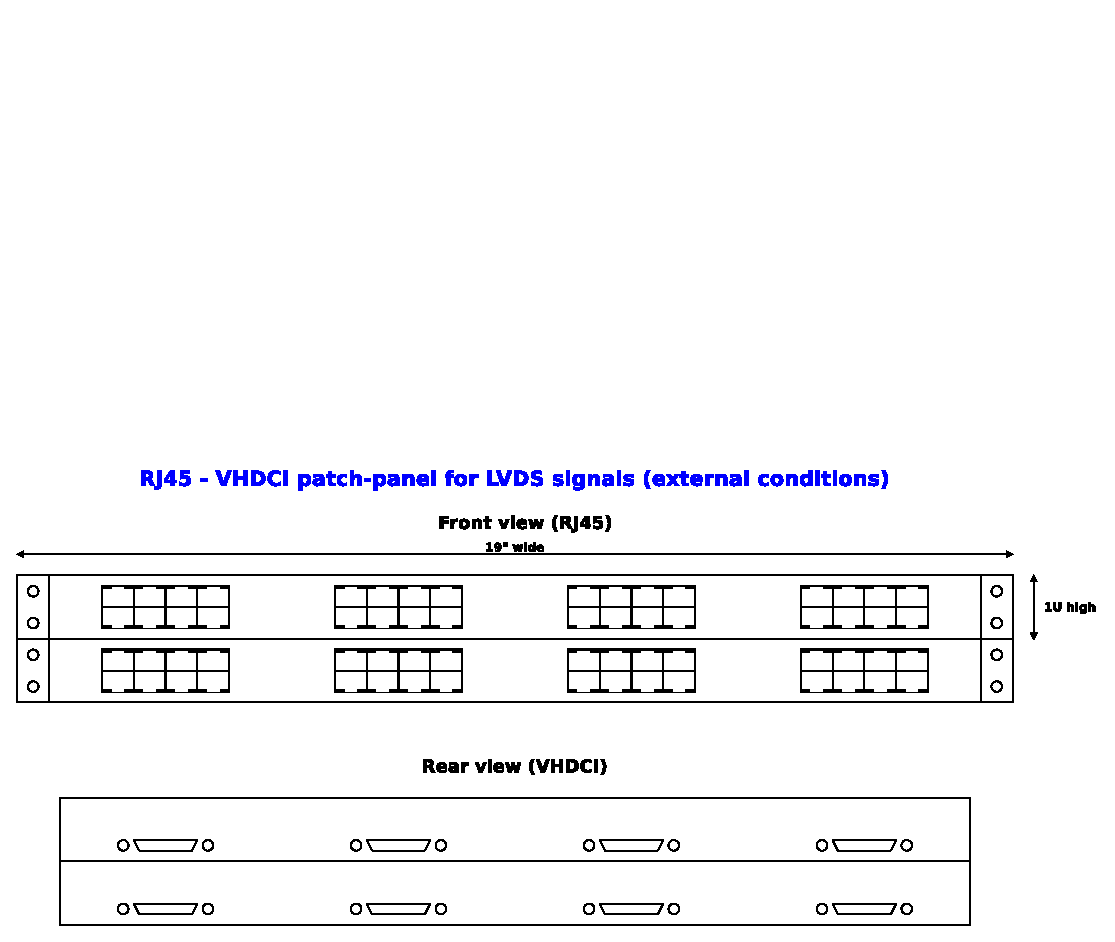
\includegraphics[width=14cm]{figures/mGT_rj45_vhdci_patch_panel}
\caption{RJ45 -VHDCI patch-panel for external conditions in \ugt-crate} 
\label{fig:com-hard:mGT_rj45_vhdci_patch_panel}
\end{figure}

\begin{figure}[htb]
\centering
\includegraphics[width=14cm]{figures/RJ45_VHDCI_Patchpanel_1}
\caption{"RJ45-VHDCI converter" back side (VHDCI)} 
\label{fig:com-hard:rj45_vhdci_patchpanel_1}
\end{figure}

\begin{figure}[htb]
\centering
\includegraphics[width=14cm]{figures/RJ45_VHDCI_Patchpanel_2}
\caption{"RJ45-VHDCI converter" front side (RJ45)} 
\label{fig:com-hard:rj45_vhdci_patchpanel_2}
\end{figure}

\begin{figure}[htb]
\centering
\includegraphics[width=14cm]{figures/RJ45_VHDCI_Patchpanel_5}
\caption{"RJ45-VHDCI converter" with cables} 
\label{fig:com-hard:rj45_vhdci_patchpanel_5}
\end{figure}

\begin{figure}[htb]
\centering
\includegraphics[width=14cm]{figures/HFMC_LVDS_mezzanine}
\caption{HFMC LVDS mezzanine} 
\label{fig:com-hard:hfmc_lvds_mezzanine}
\end{figure}

\begin{figure}[htb]
\centering
\includegraphics[width=14cm]{figures/HFMC_LVDS_mezz_GLIB}
\caption{HFMC LVDS mezzanine on GLIB2} 
\label{fig:com-hard:hfmc_lvds_mezz_glib}
\end{figure}

\clearpage

\subsection{Arrangement of \ugt-crate and patch-panels in \ugt-rack}\label{sec:com-hard:cabling_mgt_rack}

The arrangement and the cabling between \ugt-crate and patch-panels is \textbf{very preliminary}. For exact arrangement all the dimension are to known.\\
In Figure \ref{fig:com-hard:mGT_rack_cabling} one can see, how the cabling between the patch-panels and the \ugt-crate could be done. On the back side of the \ugt-rack
all the "external" cables are connected to the patch-panels, 64 RJ45-cables for the external condition data (max. 256 bits), 2 MTP48 optical cables with 36 LC connectors
for Calo-L2 data to \ugt, 1 MTP48 optical cable with 36 LC connectors for Calo-L2 data to \ugmt and 3 MTP12 optical cables with 12 LC connectors for data from Barrel TF,
Forward TF and Overlap TF. In addition there is a "internal" cable from \ugmt to optical patch-panel for \ugmt output data to \ugt (1 MTP48 optical cable with 36 LC connectors).\\
The connections from the patch-panels to \ugt-crate are made with 8 VHDCI 68 cables to HFMC (mezzanine board) on GLIB3 and with 8 MTP48 optical cables with 36 LC connectors
to MP7 modules (6 for \ugt, 2 for \ugmt). See also Section \ref{sec:com-hard:external_cond} and Figure \ref{fig:com-hard:mGT_mGMT_fiber_optical_patch}.\\
In Figure \ref{fig:com-hard:mGT_rack_cabling_views} a scheme of the arrangement of \ugt-crate and patch-panels within the \ugt-rack is shown in three views (top, front and back).\\
\textbf{Remark}: if there is not enough space for a height of 10U (7U \ugt-crate, 2U "RJ45-VHDCI patch-panel" and 1U "\finor patch-panel"),
the "RJ45-VHDCI patch-panel" could be arranged behind the \ugt-crate at the same height of top as the top of the \ugt-crate, which would need only 8U.

\begin{figure}[htb]
\centering
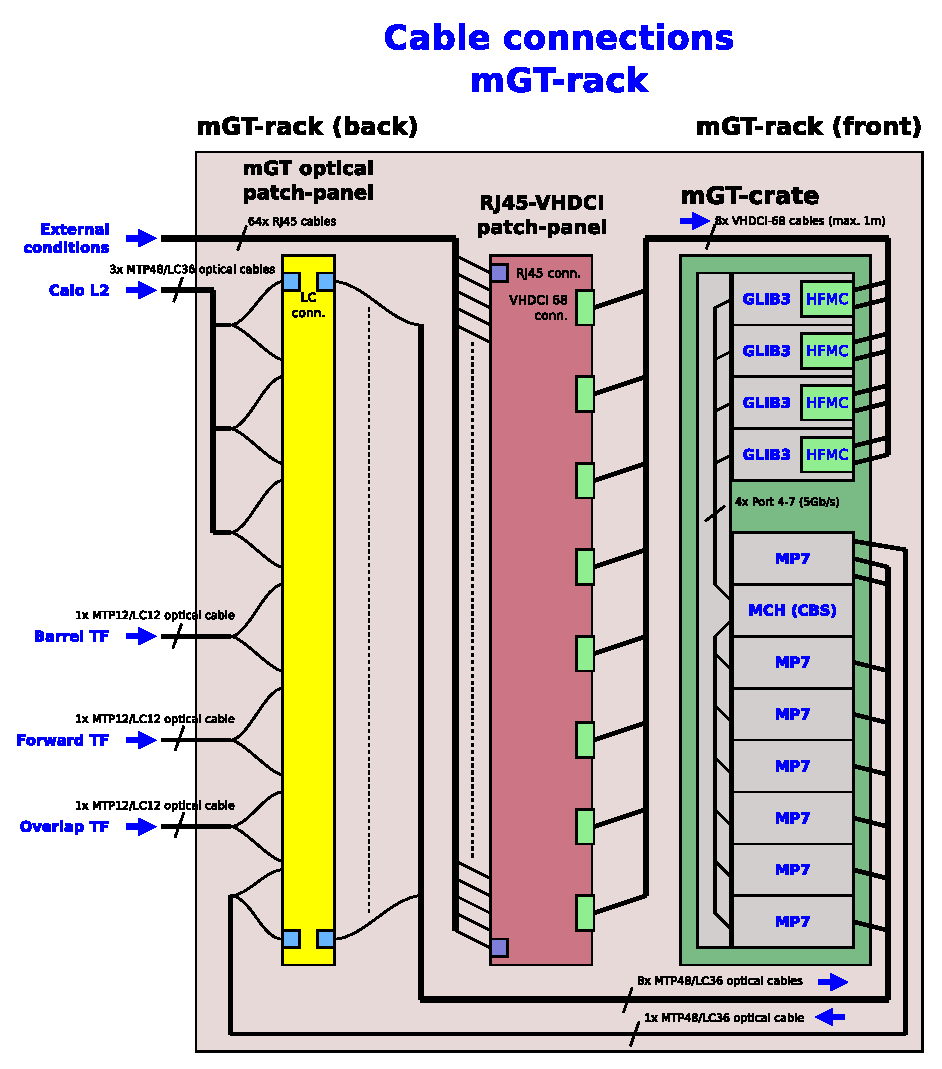
\includegraphics[width=14cm]{figures/mGT_rack_cabling}
\caption{Cable connections in \ugt-rack (top view)} 
\label{fig:com-hard:mGT_rack_cabling}
\end{figure}

\clearpage

\begin{figure}[htb]
\centering
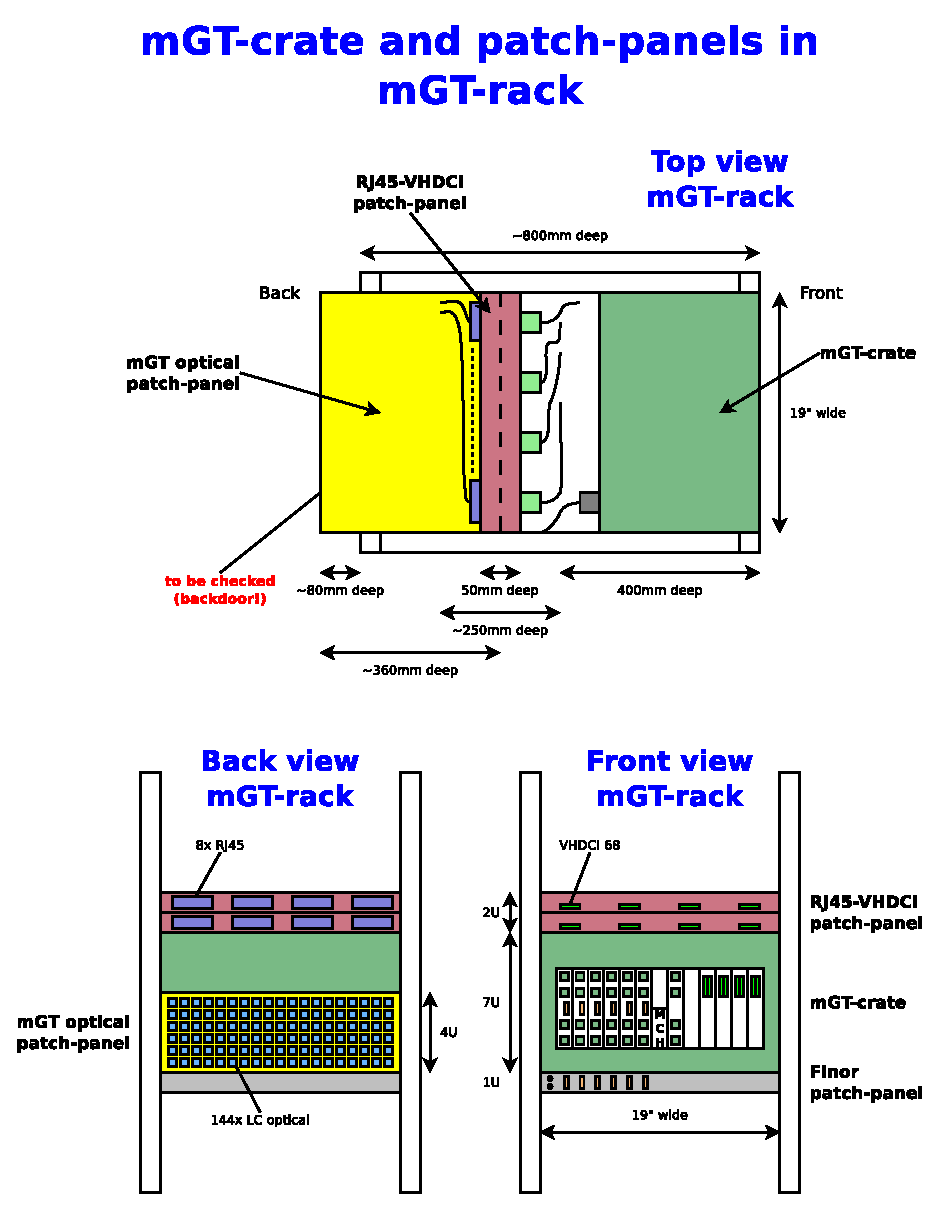
\includegraphics[width=14cm]{figures/mGT_rack_cabling_views}
\caption{Views of \ugt-crate and patch-panels in \ugt-rack} 
\label{fig:com-hard:mGT_rack_cabling_views}
\end{figure}
